\chapter{Detailed System Design}
\label{chap:system_design}

This chapter provides a comprehensive exposition of the system's detailed design, articulating the architectural decisions, methodologies, and technological implementations that underpin the platform. The design philosophy centers on leveraging a modern, serverless architecture to achieve scalability, maintainability, and rapid development. Each section adopts a problem-solution paradigm, presenting a specific technical challenge encountered during the development lifecycle, followed by a detailed description of the implemented solution, its rationale, and its advantages.

\section{System Architecture Overview}
\label{sec:system_architecture_overview}

The platform's architecture is a system comprising several loosely coupled components, orchestrated to deliver a seamless data annotation experience. The high-level architecture, as depicted in Figure \ref{fig:system_architecture}, segregates responsibilities into four primary domains: the client-side frontend, the serverless backend, external service integrations, and a reverse proxy layer for routing and security.

\begin{figure}[H]
    \centering
    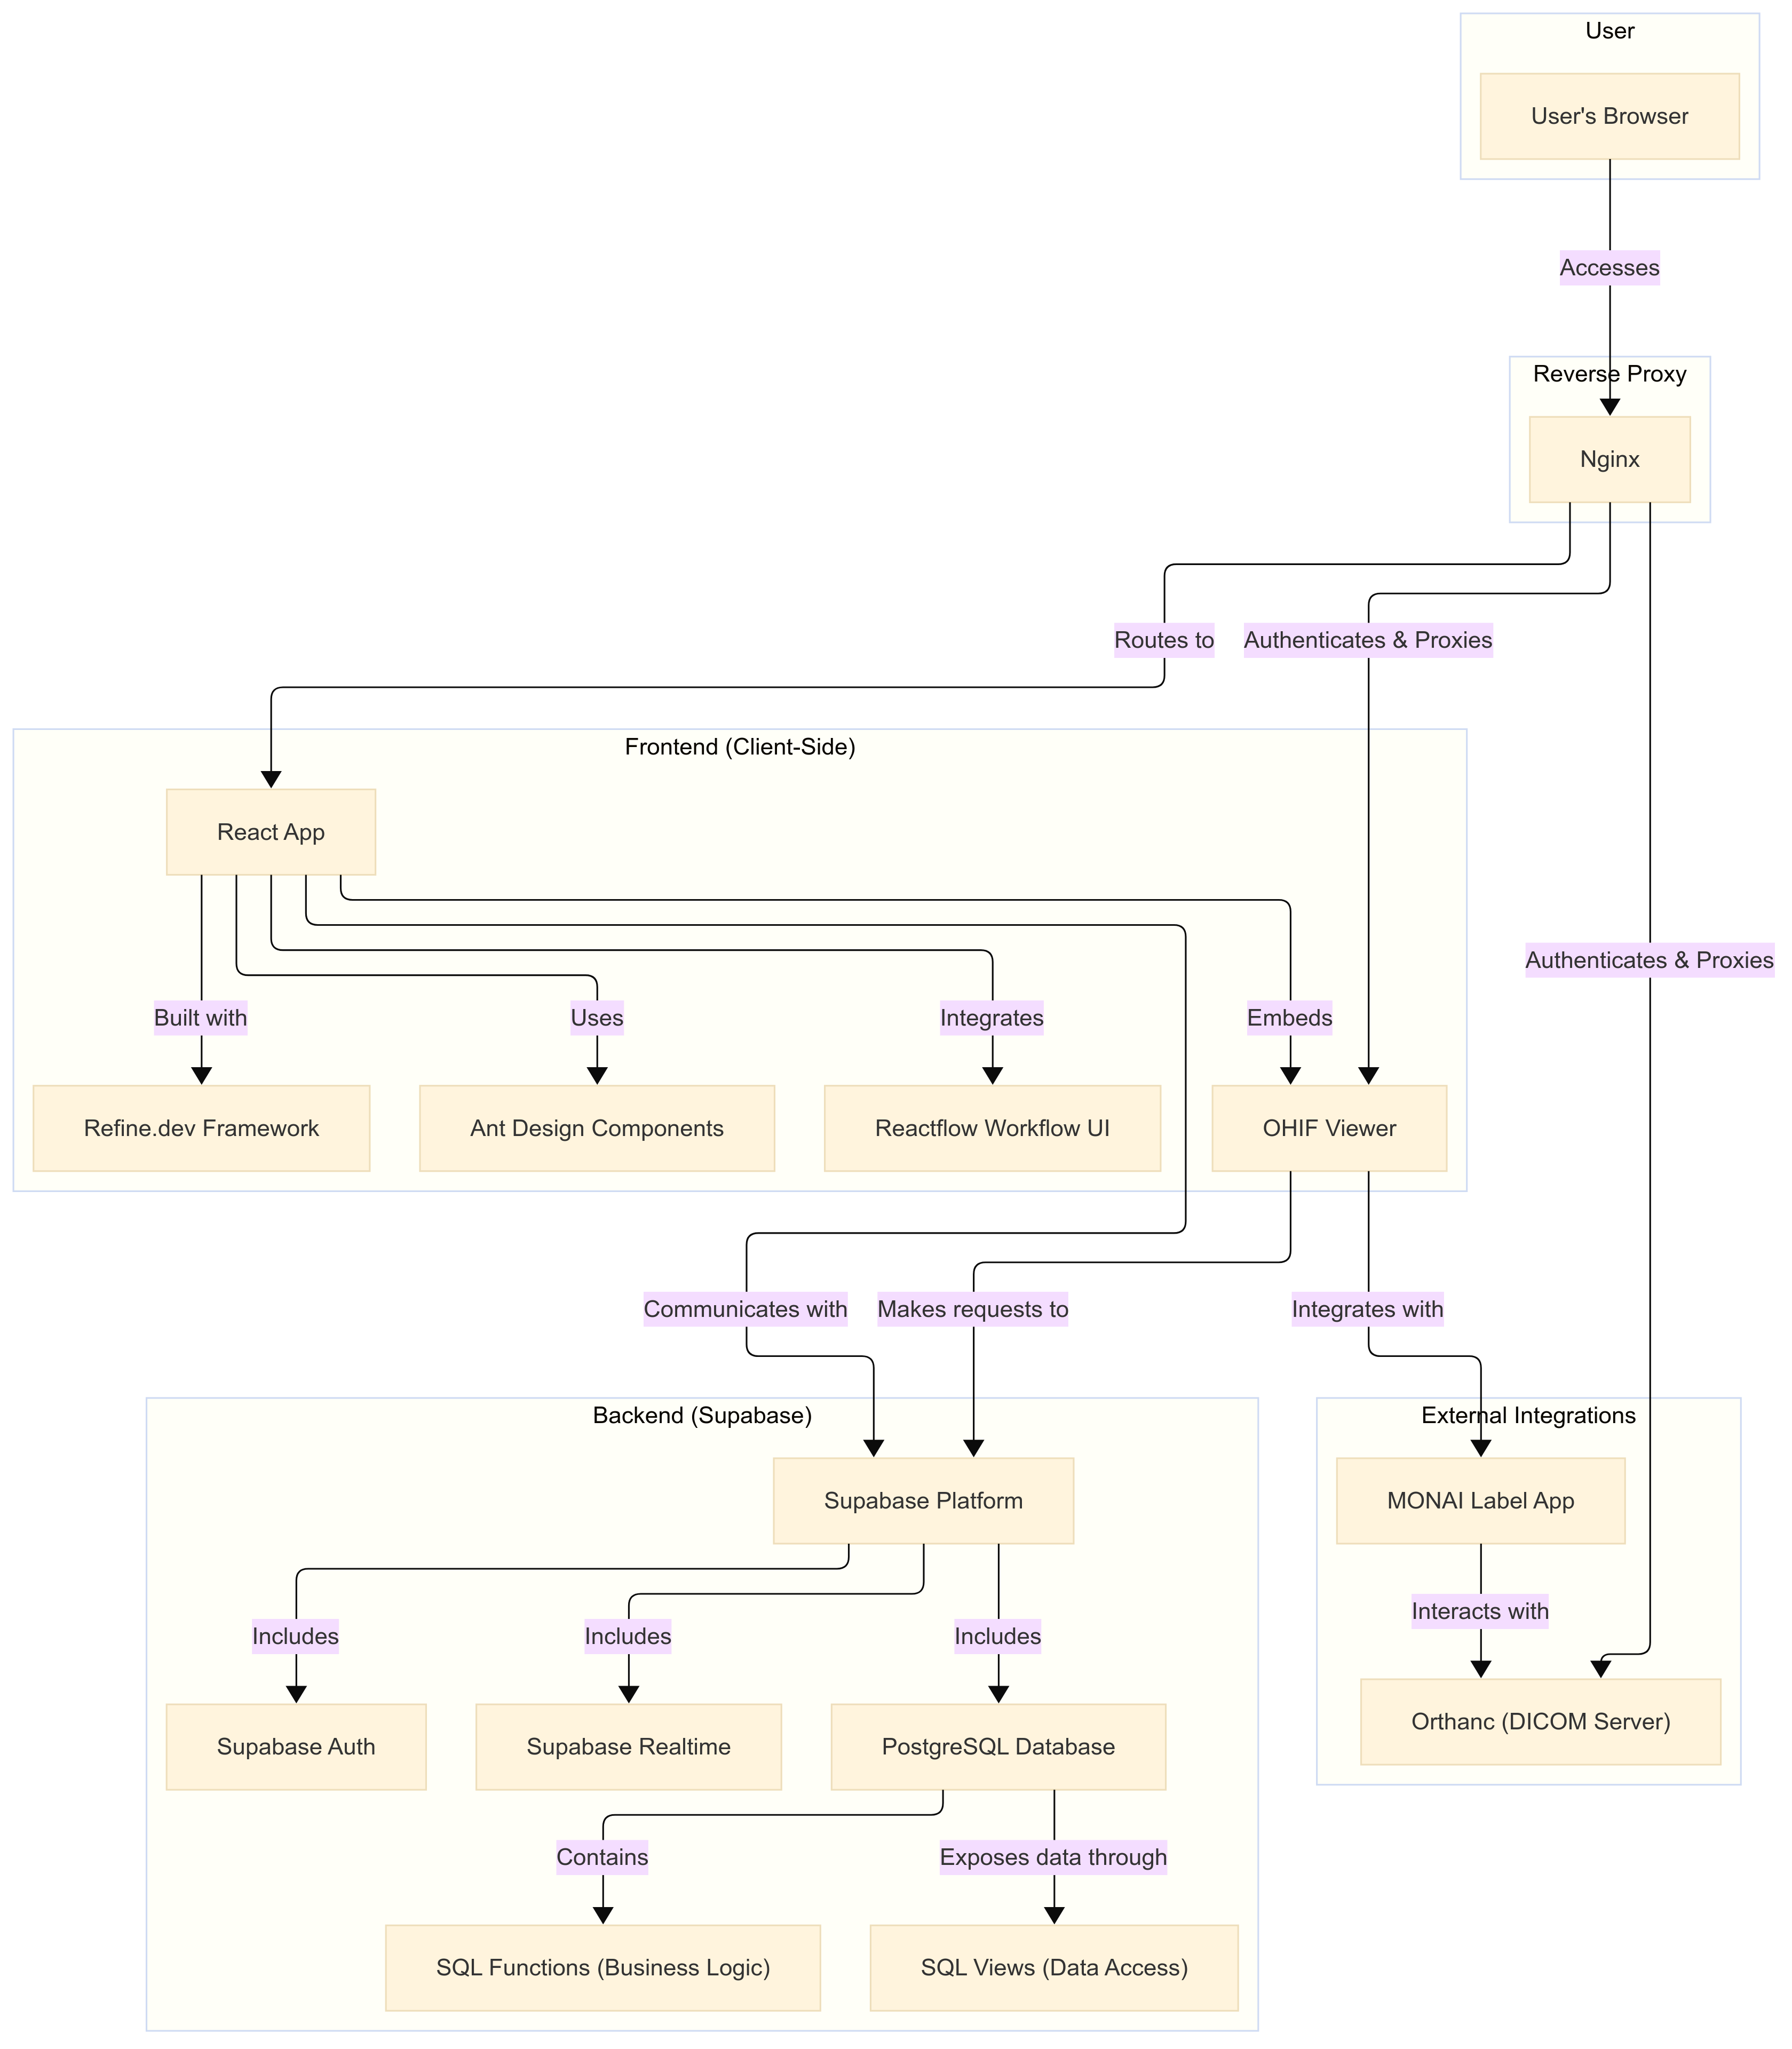
\includegraphics[width=1\linewidth]{content//resources//images//chap4-system-design/architecture.png}
    \caption{High-Level System Architecture Diagram.}
    \label{fig:system_architecture}
\end{figure}

The frontend is a single-page application (SPA) built with React, responsible for all user interactions. The backend is implemented entirely on the Supabase platform, utilizing its PostgreSQL database, authentication services, and real-time capabilities. This backend-as-a-service (BaaS) model obviates the need for traditional server management. Key external integrations, such as the OHIF Viewer for DICOM rendering and MONAI Label for AI-assisted annotation, are incorporated to provide specialized functionality. An Nginx reverse proxy serves as the entry point to the system, managing request routing and centralizing authentication concerns. The subsequent sections will deconstruct this architecture, providing a granular analysis of each component's design.

\section{Frontend Architecture}
\label{sec:frontend_architecture}

The frontend architecture is engineered for rapid development, maintainability, and a high-quality user experience. The design addresses two fundamental challenges in modern web application development: the overhead of building standard application features and the complexity of client-side state management.

\subsection{Accelerating Development with a Headless Framework}
\label{subsec:accelerating_development}

\subsubsection{Problem: Boilerplate and Scaffolding Overhead}
Developing a data-intensive application from the ground up necessitates a disproportionate amount of engineering effort dedicated to repetitive, boilerplate code rather than unique business features. For each distinct data entity—such as \texttt{projects}, \texttt{tasks}, or \texttt{users}—a developer must manually implement a full suite of standard features. This includes a view to list all items, a form to create new ones, views to display and edit item details, and the logic to delete them. This pattern, commonly known as Create, Read, Update, Delete (CRUD), extends beyond data operations to include user authentication flows (login, logout, registration), system notifications, navigation menus, and breadcrumbs.

Without a structured framework, this leads to a proliferation of nearly identical yet subtly different code blocks. A developer might write a custom React hook for fetching project data, another for task data, and so on. Each implementation would require its own state management (`useState`), effect handling (`useEffect`), and API call logic. This approach is not only exceedingly time-consuming but also highly susceptible to inconsistencies in implementation, error handling, and loading state management, ultimately degrading code quality and maintainability.

\subsubsection{Solution: Adoption of the Refine.dev Framework}
The platform leverages the \texttt{refine.dev} framework, a headless, React-based framework designed specifically to abstract these common application patterns. Its core architectural concept is the \textbf{resource}, a declarative object that defines a data entity and its associated behaviors.

By defining a resource, the developer provides \texttt{refine.dev} with the metadata required to automate a vast array of functionalities. A resource definition for "projects" is as follows:
\begin{lstlisting}[language=c]
<Refine
    dataProvider={...}
    notificationProvider={...}
    routerProvider={...}
    authProvider={...}
    resources={[
        {
            name: "projects",
            list: "/projects",
            create: "/projects/create",
            edit: "/projects/edit/:id",
            show: "/projects/show/:id",
            meta: { canDelete: true }
        },
        // ... other resources like "tasks", "users"
    ]}
>
    {/* Application components */}
</Refine>
\end{lstlisting}
This single, declarative definition unlocks a suite of powerful, interconnected features, forming the backbone of the application:
\begin{itemize}
    \item Standardized Data Hooks provide high-level data hooks (\texttt{useList}, \texttt{useOne}, \texttt{useCreate}, \texttt{useUpdate}, \texttt{useDelete}) that are pre-configured to communicate with the backend \texttt{dataProvider}. This eliminates the need to write manual fetching logic for each resource.
    \item Automated Routing enables the framework to generate necessary routes for the \texttt{list}, \texttt{create}, \texttt{edit}, and \texttt{show} pages, integrating seamlessly with its \texttt{routerProvider}.
    \item Dynamic UI Generation works with UI libraries like Ant Design where \texttt{refine.dev} automatically generates side-menu navigation links and breadcrumbs for each resource, ensuring a consistent and intuitive user experience.
    \item Integrated Authentication leverages the framework's \texttt{authProvider} to handle login/logout flows and protect routes, redirecting unauthenticated users automatically.
    \item Centralized Notifications leverage the \texttt{notificationProvider} to dispatch system-wide notifications for success or error events during data operations.
\end{itemize}

This resource-centric paradigm abstracts away the low-level implementation details of application infrastructure. It enabled the development team to bypass thousands of lines of boilerplate code and focus engineering effort on high-value, domain-specific features.

\subsection{Efficient Data Caching and State Synchronization}
\label{subsec:efficient_caching}

\subsubsection{Problem: Inefficient Data Fetching and UI Inconsistency}
Managing server state—data fetched from a remote source—is a formidable challenge in any complex SPA. Without a sophisticated caching strategy, applications suffer from poor performance, redundant network traffic, and UI inconsistencies. Two common anti-patterns demonstrate this problem:

\begin{enumerate}
    \item \textbf{Component-Level Fetching and Request Waterfalls}: The most direct approach involves each component fetching its own data using `useEffect`. This leads to perceptible latency as a parent component fetches data, and then its child components, upon rendering, initiate their own separate data fetches. Furthermore, if multiple unrelated components on the same page require the same data (e.g., the current user's profile), they will each make a redundant API call for that data, wasting bandwidth and backend resources.
    \item \textbf{Manual Caching with Global State}: To solve redundancy, developers often implement a manual caching layer using a global state library like Redux. Data is fetched once and stored centrally. While this prevents duplicate requests, it introduces immense boilerplate for actions, reducers, and selectors. More critically, the cache quickly becomes stale. If a user updates their profile in one part of the app, it becomes the developer's manual responsibility to dispatch an action to update the cache and ensure all subscribed components re-render. This manual cache invalidation is a frequent source of bugs, leading to inconsistent UIs displaying outdated information.
\end{enumerate}

\subsubsection{Solution: Declarative Caching and Automated Invalidation with TanStack Query}
The \texttt{refine.dev} framework addresses these challenges by integrating TanStack Query as its default server-state management engine. This library provides a robust, out-of-the-box solution that automates caching, background updates, and state synchronization.

When fetching a resource \texttt{projects} using a hook like \texttt{useList("projects")}, TanStack Query fetches the data and stores it in a global, in-memory cache under a unique query key, in this case, \texttt{["projects"]}. Any subsequent call to \texttt{useList("projects")} from any other component will instantly receive the cached data, eliminating redundant network requests. The cache's behavior is controlled by key parameters:
\begin{itemize}
    \item \textbf{\texttt{staleTime}}: Dictates the duration for which cached data is considered "fresh" and can be served without a network call.
    \item \textbf{\texttt{cacheTime}}: Dictates how long inactive (unmounted) data is retained in memory before being garbage collected.
\end{itemize}
The most significant architectural advantage is its automated approach to synchronization via \textbf{query invalidation}. After a mutation (e.g., a user updates a project via the \texttt{useUpdate} hook), \texttt{refine}'s data provider automatically calls \texttt{queryClient.invalidateQueries(["projects"])}. This action does not naively trigger a refetch. Instead, it marks all data associated with the \texttt{['projects']} key as stale. TanStack Query then intelligently and automatically refetches the data only for the currently mounted components that are subscribed to that query.

This strategy obviates the need for the "prop drilling" anti-pattern, where a \texttt{refetch} function must be passed down through multiple component layers. The component triggering the mutation remains blissfully unaware of which other components display the data. It simply invalidates the relevant data key, and the framework guarantees UI consistency across the entire application. This declarative approach radically simplifies state management, reduces bugs, and improves application performance.





\section{Backend Architecture and Workflow Orchestration}
\label{sec:backend_architecture}

The backend architecture is founded on the principle of a "logic-intensive database" wherein complex business rules, data access policies, and asynchronous processes are encapsulated directly within PostgreSQL. This approach, facilitated by Supabase, minimizes external dependencies and centralizes the system's core logic.

\subsection{Secure and Abstracted Data Access via Views and Functions}
\label{subsec:secure_data_access}

\subsubsection{Problem: Direct Table Exposure and Logic Duplication}
Exposing raw database tables directly via an API is a significant security risk and a poor architectural practice. It tightly couples the frontend application to the physical data schema, making future schema migrations brittle and error-prone. Furthermore, essential business logic and validation rules (e.g., "a new project must be assigned to the user who created it," or "a task's status can only transition from PENDING to COMPLETED") would need to be re-implemented in every client or middleware that interacts with the data, leading to code duplication and inevitable inconsistencies.

\subsubsection{Solution: A Multi-Layered Abstraction with PostgreSQL Views and Functions}
To address this, the backend employs a robust abstraction layer within the database itself.
\begin{itemize}
    \item \textbf{Core Tables}: The fundamental data is stored in "private" tables, prefixed with an underscore (e.g., \texttt{\_projects}, \texttt{\_tasks}). These tables are never directly exposed to the `API`.
    \item \textbf{Security Views}: For data retrieval (Read operations), PostgreSQL views are created (e.g., \texttt{projects}, \texttt{tasks}). These views act as a stable public interface for the frontend. They are defined with \texttt{WITH (security\_invoker = true)} and are governed by Supabase's Row-Level Security (RLS) policies, ensuring that users can only see the data they are permitted to access.
    \item \textbf{SQL Functions as Atomic Transactions}: For all data mutations (Create, Update, Delete), dedicated PostgreSQL functions are implemented. For standard resource operations, these functions follow a strict naming convention (e.g., \texttt{projects\_create}). For more complex business processes that do not fit the CRUD model, such as "submitting a task for review" or "initiating a consensus check," the platform leverages \texttt{refine.dev}'s \texttt{useCustomMutation} hook. This allows the frontend to directly invoke a specific SQL function via RPC, ensuring that all logic remains centralized, atomic, and secure within the database.
\end{itemize}

This design effectively decouples the physical schema from the API, enforces security at the data layer, and guarantees that business logic is executed atomically and consistently, irrespective of the client initiating the request.

\subsection{Asynchronous Workflow Automation Engine}
\label{subsec:workflow_automation}

\subsubsection{Problem: The Cognitive Gap Between User Interface and Backend Complexity}
A fundamental challenge in designing user-friendly workflow builders lies in abstracting backend complexity without creating ambiguity. Data annotation platforms often require sophisticated processes like consensus, where multiple annotators work in parallel before their results are algorithmically compared. Leading platforms in the space often represent such complex operations as a single, monolithic "black box" node on the UI canvas.
\begin{figure}[H]
    \centering
    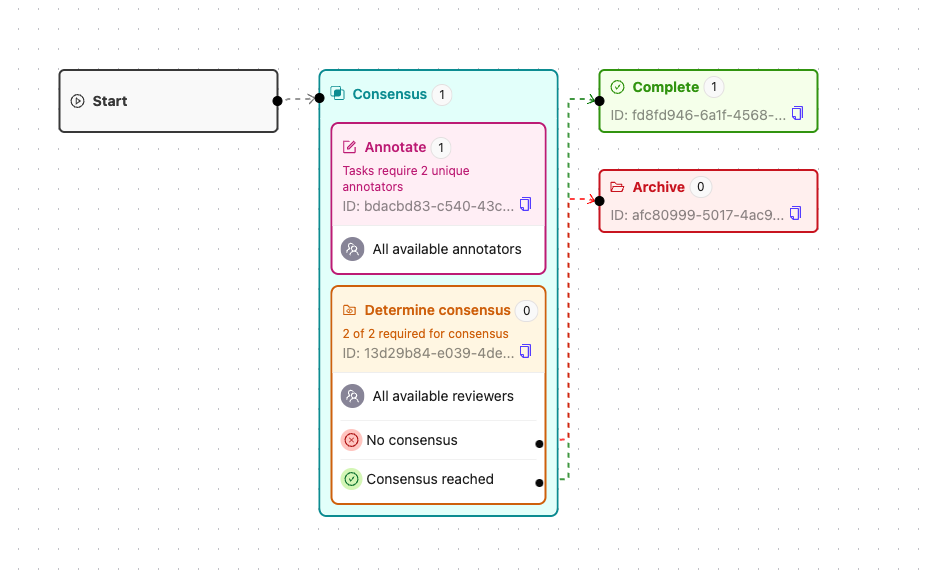
\includegraphics[width=0.8\textwidth]{content/resources/images/chap4-system-design/blackbox.png}
    \caption{Example of a "black box" consensus node in a workflow builder. The internal logic and flow are not visually represented.}
    \label{fig:blackbox_ui}
\end{figure}

Figure \ref{fig:blackbox_ui} show that user might be presented with a single "Consensus" node. While functionally powerful, this high level of abstraction can obscure the underlying process flow from the very users it is meant to empower—project managers and non-technical stakeholders. The user configures parameters within this single node, but the actual sequence of events—the creation of parallel annotation tasks, the aggregation of results, and the conditional logic for agreement or disagreement—remains implicit and invisible. This lack of transparency can lead to confusion, making it difficult for users to audit the workflow's logic, predict its behavior, or understand why a task has progressed in a certain way without deep system knowledge. The core problem is the cognitive gap between the simplified UI and the complex reality of the backend orchestration.


\subsubsection{Solution: Cron-Driven Orchestration from a Declarative Database Model}
The platform addresses this challenge by implementing a powerful and extensible workflow engine entirely within PostgreSQL, driven by scheduled cron jobs. This engine translates the declarative, visual workflow definition stored in the database into concrete, asynchronous actions.

The bridge between the visual interface and the backend logic is the \texttt{\_workflow\_stages} table. When a user designs a workflow using the \texttt{xyflow} frontend library, each node on the canvas corresponds to a row in this table. A "Consensus" node, for example, is stored with its \texttt{type} field set to \texttt{'CONSENSUS'} and its specific parameters, such as the number of required annotators, stored in a \texttt{custom\_config} JSONB field (e.g., \texttt{\{"annotators\_required": 3\}}).

The orchestration is then executed by a targeted cron job at the precise moment a task enters this stage, as illustrated in Figure \ref{fig:workflow_engine_flow}:
\begin{enumerate}
    \item \textbf{Stage Entry and Assignment}: When a task successfully completes a preceding stage, a new record is created in the \texttt{\_task\_assignments} table. This record links the task to the "Consensus" stage's ID and assigns it to a special "virtual user" named \texttt{CONSENSUS}. This assignment acts as a flag, signaling that the task is ready for automated processing.

    \item \textbf{Cron Job Execution}: A PostgreSQL cron job, \texttt{workflow\_consensus()}, is scheduled to run periodically (e.g., every minute). This function's sole responsibility is to query the \texttt{\_task\_assignments} table for any pending tasks assigned to the \texttt{CONSENSUS} virtual user.

    \item \textbf{Dynamic Sub-Task Generation}: Upon finding such a task, the cron function executes the core orchestration logic. It reads the \texttt{custom\_config} from the associated workflow stage to determine that three annotators are needed. It then dynamically creates three new, parallel annotation sub-tasks, assigns them to available human annotators, and updates the parent task's status to a holding state, awaiting the completion of these children.
\end{enumerate}

This design effectively decouples the workflow's definition from its execution. New, complex stage types can be introduced into the system with minimal effort: a developer simply needs to create a new frontend node component and a corresponding backend cron function to handle the logic for that stage's specific \texttt{type}. This approach provides a robust, scalable, and fully serverless workflow engine that is both powerful in its execution and simple to extend.


\section{Infrastructure and Security}
\label{sec:infrastructure_security}

\subsection{Unified Authentication Across Micro-Frontends}
\label{subsec:unified_authentication}

\subsubsection{Problem: Disparate Authentication States}
The system's architecture integrates the OHIF Viewer as an embedded component, which effectively acts as a micro-frontend within the main application. A naive implementation would lead to significant authentication challenges. Each "frontend" (the main app and the viewer) would need to manage its own authentication state. This could require the user to log in twice or involve complex, insecure token-passing mechanisms (e.g., using \texttt{postMessage} to send a JWT to the viewer's iframe). This approach creates a fragmented user experience and enlarges the attack surface for vulnerabilities like token interception.

\begin{figure}[H]
    \centering
    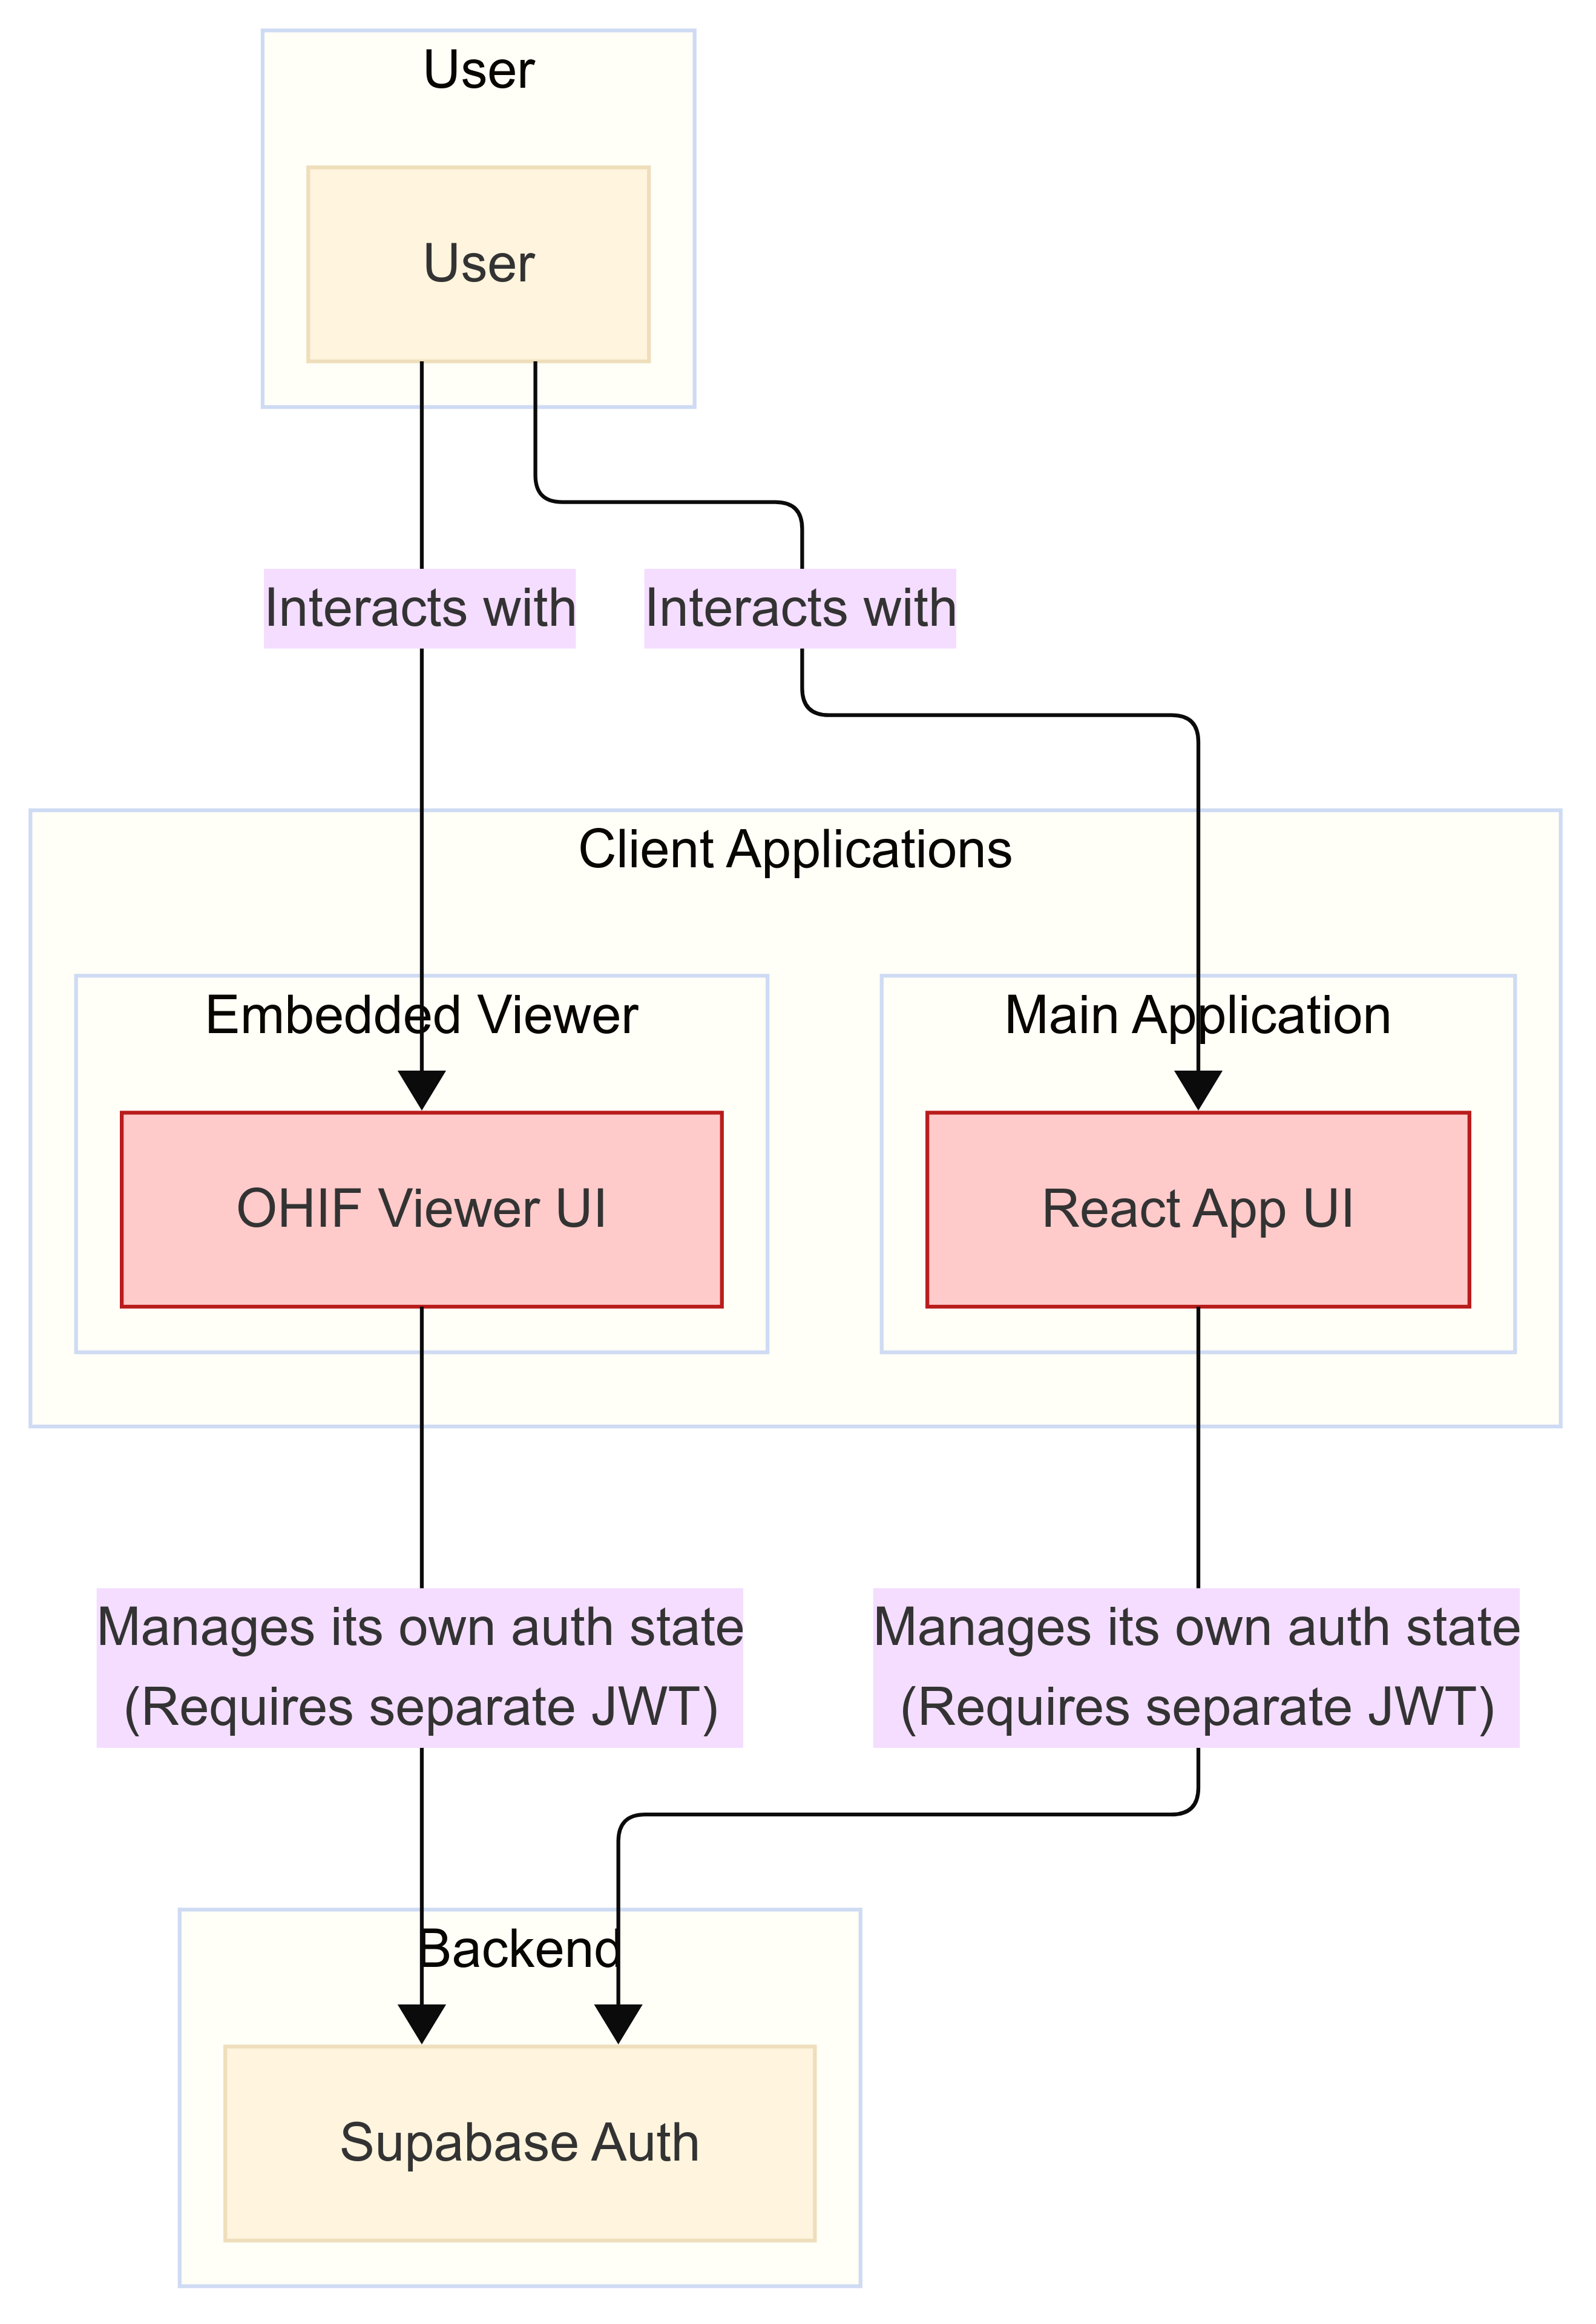
\includegraphics[width=\textwidth]{content/resources/images/chap4-system-design/Problematic Disparate Authentication Architecture.png}
    \caption{Problematic Disparate Authentication Architecture.}
    \label{fig:disparate_auth}
\end{figure}

\subsubsection{Solution: Centralized Authentication via Nginx Reverse Proxy}
The chosen solution was to centralize authentication at the infrastructure level using Nginx as a reverse proxy and authentication gateway. This pattern, shown in Figure \ref{fig:unified_auth}, removes the burden of authentication enforcement from the individual client applications.

\begin{figure}[H]
    \centering
    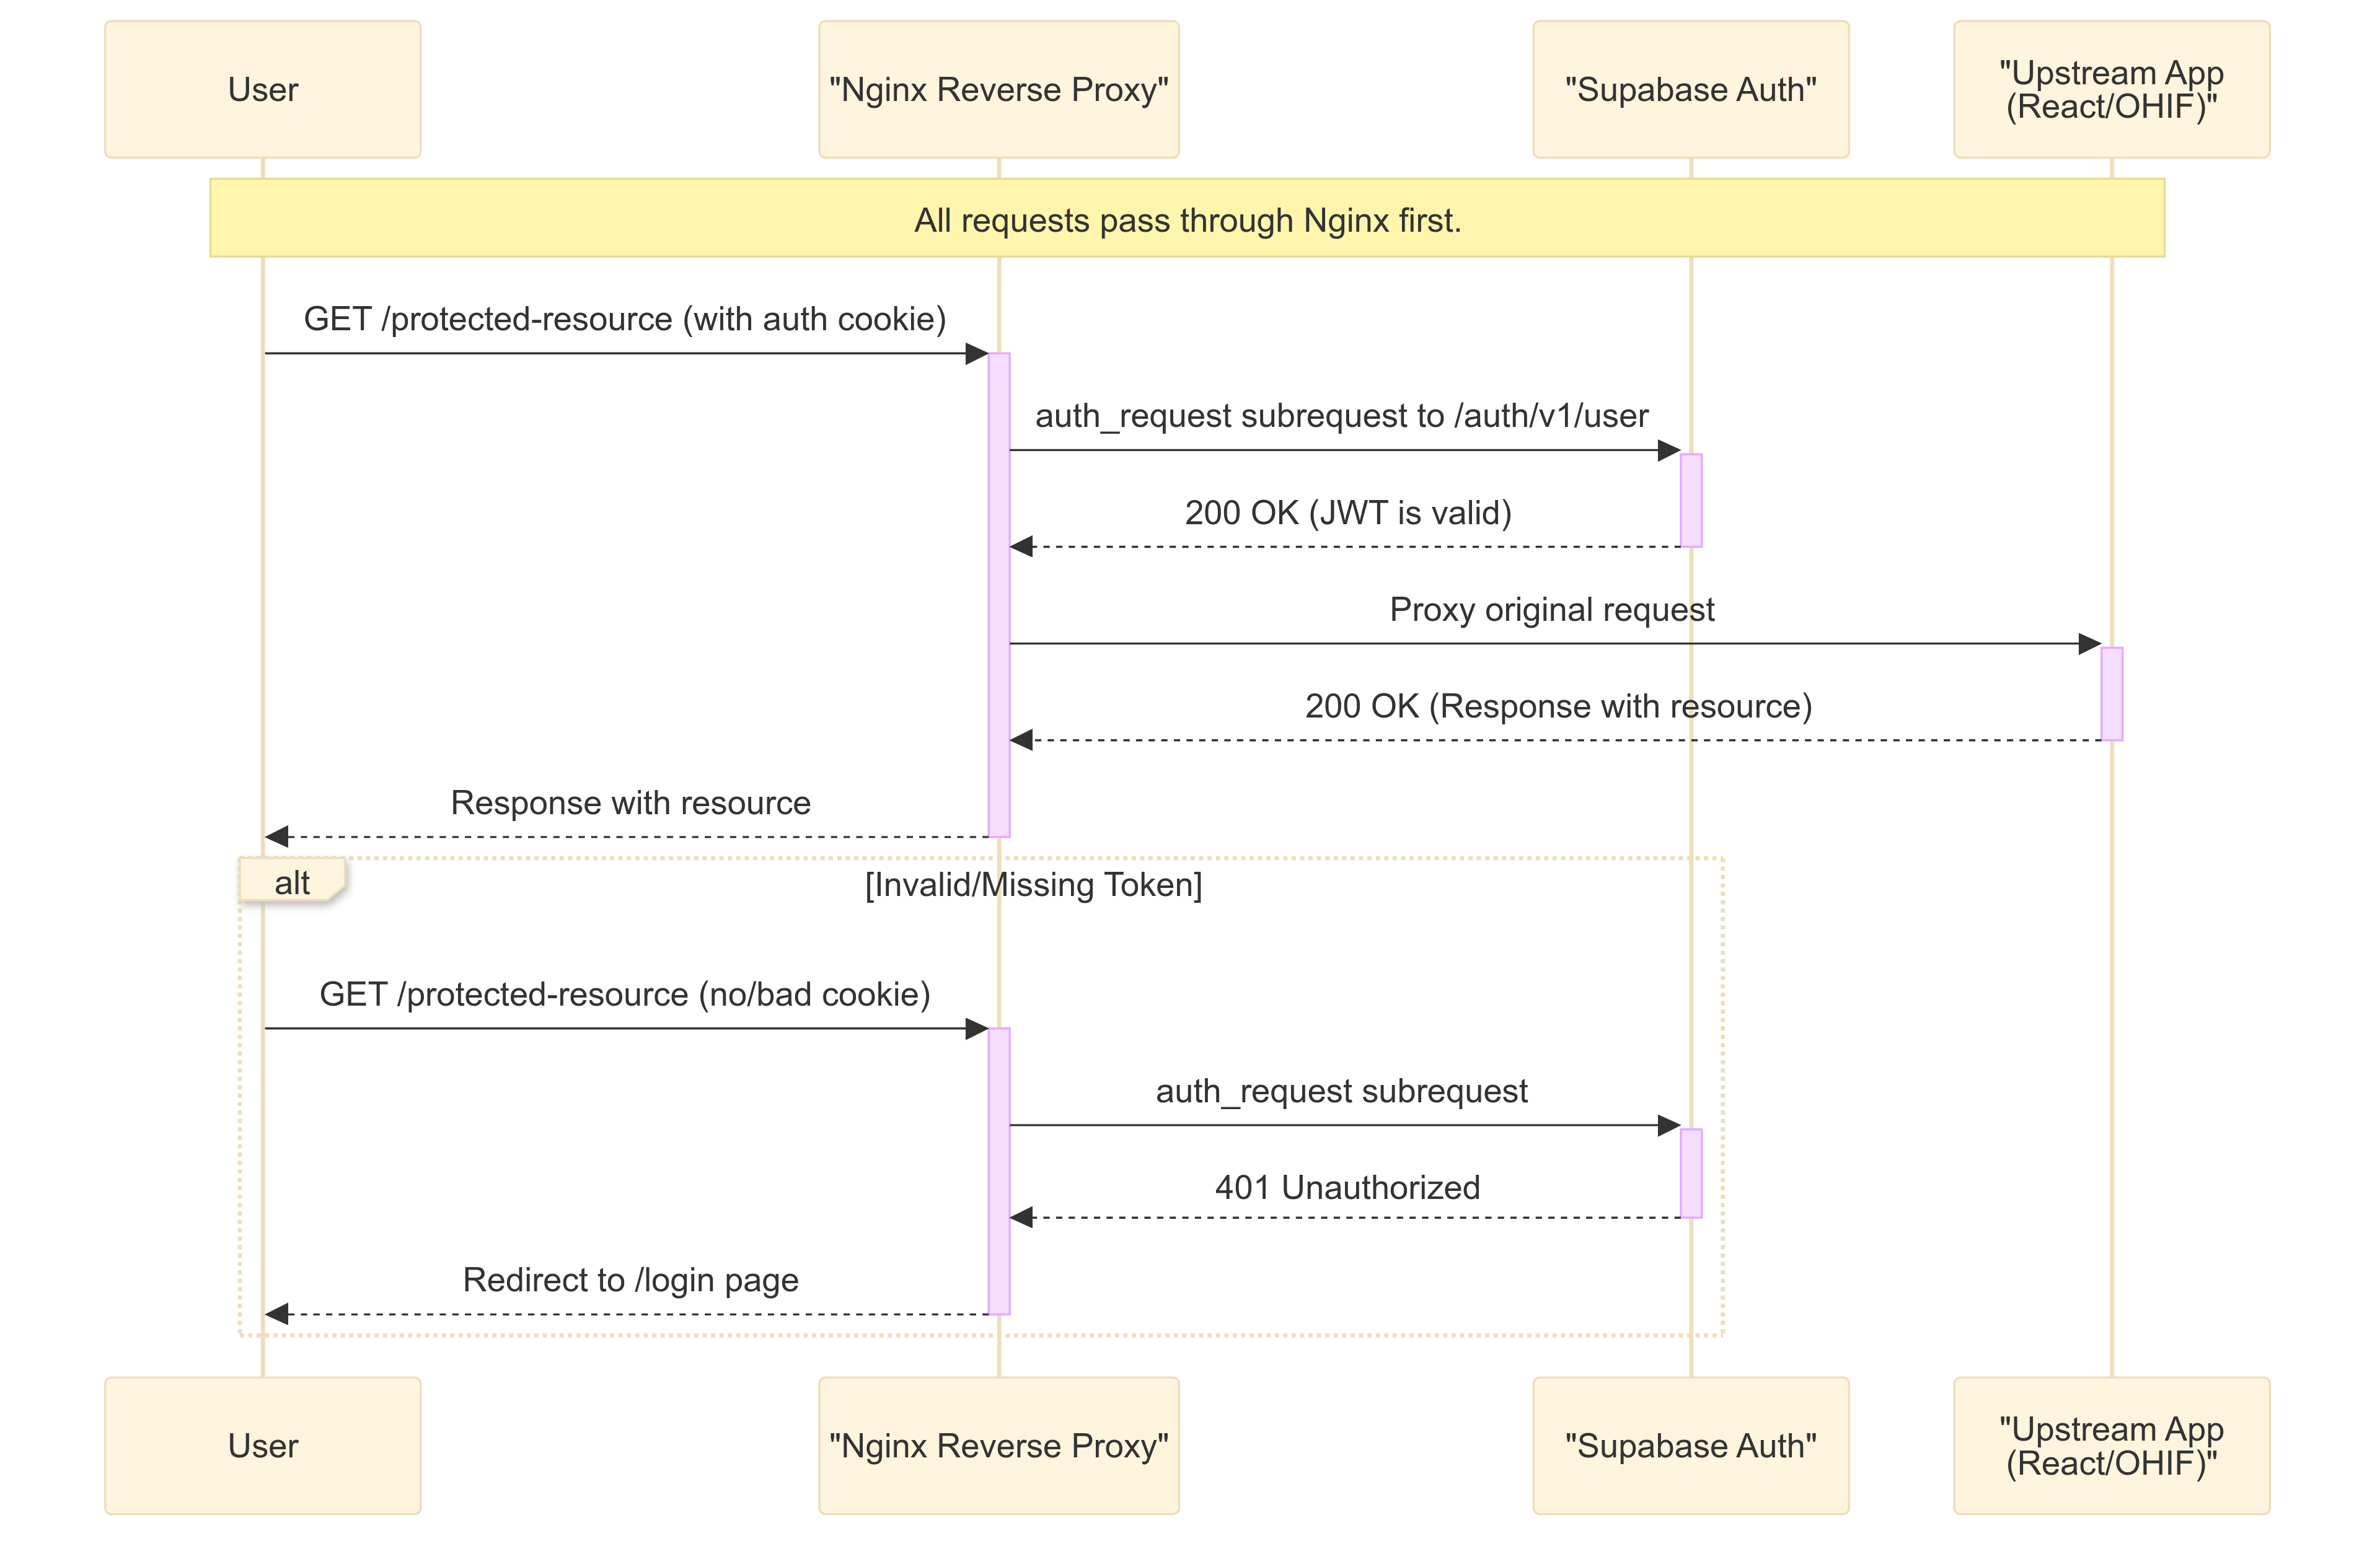
\includegraphics[width=\textwidth]{content/resources/images/chap4-system-design/Centralized Authentication via Nginx Reverse Proxy.png}
    \caption{Centralized Authentication via Nginx Reverse Proxy.}
    \label{fig:unified_auth}
\end{figure}

The request flow is as follows:
\begin{enumerate}
    \item The user's browser makes a request to any part of the application.
    \item Nginx, as the sole entry point, intercepts the request and inspects the Supabase JWT stored in a secure, HttpOnly cookie.
    \item Nginx uses the \texttt{auth\_request} directive to make an internal subrequest to a protected Supabase endpoint (e.g., /auth/v1/user).
    \item \textbf{If the token is valid}, the subrequest returns a 200 OK status, and Nginx proxies the original request to the appropriate upstream service (the main React application or the OHIF viewer).
    \item \textbf{If the token is invalid or absent}, the subrequest returns a 401 Unauthorized status, and Nginx immediately redirects the user to the login page without the request ever reaching the downstream applications.
\end{enumerate}

This configuration hugely simplifies the frontend code. Neither the main application nor the OHIF integration needs to contain logic to protect its routes; they can trust that any request they receive has already been authenticated by the Nginx gateway. This creates a more secure, maintainable, and robust authentication system.